\section{Data}
\label{sec:data}

\subsection{Hourly Load of the SIN Subsystems}
The SIN is divided into four interconnected subsystems: North (N), Northeast (NE), South (S), and Southeast/Center-West (SE), the latter accounting for more than half of the national demand. Our primary data set is the hourly load curve published by ONS in its open-data portal~\cite{ons_opendata}, which reports the average hourly load (MWh/h, i.e., average MW) per subsystem. We use the period from January~1, 2012 to November~4, 2026, i.e., \NHours{} hourly observations per subsystem. Timestamps are in Bras\'ilia legal time; the hours skipped at the start of daylight-saving time (abolished in 2019) appear as missing values.

\subsection{Verified Global Load, Behind-the-Meter Generation, and the Official Forecast}
To compare our models with the forecasts actually used in system operation, we also retrieved, through the public ONS load API~\cite{ons_apicarga}, two half-hourly series: (i) the \emph{verified global load} (\emph{carga global verificada}), available from 2020 onwards, which includes an estimate of the energy produced by behind-the-meter MMGD and is also reported together with this estimate; and (ii) the \emph{programmed global load} (\emph{carga global programada}), i.e., the official day-ahead load forecast used by ONS in the daily operation programming, available from March 2021 onwards. Both series were converted from UTC to Bras\'ilia time and aggregated to hourly means to match the hourly curve. Because the definitions of the two ONS products differ slightly, every comparison with the official forecast (Section~\ref{sec:res_ons}) is performed on the verified global load, which is the quantity the official forecast targets.

\subsection{Pre-processing}
Missing values, non-positive values, and isolated spikes or dips deviating by more than 20\% from a centred 5-hour rolling median were replaced; short gaps were linearly interpolated and whole missing days were filled with the profile of the previous week rescaled to the local level. Most flagged values correspond to daylight-saving transitions, recording failures, and major blackouts (e.g., March~21, 2018 and August~15, 2023), which are not forecastable from load data. Overall, \CleanedPct\% of the entries were modified. The same procedure was applied to the verified global load.

\subsection{Characteristics of the Series}
Table~\ref{tab:data} summarises the series. Demand grew strongly over the study period, especially in the North, driven by new industrial consumers and electrification, and in all subsystems after 2020. Fig.~\ref{fig:data}(a) shows the annual mean load and Fig.~\ref{fig:data}(b) shows the share of the global load supplied by behind-the-meter MMGD between 11:00 and 14:59, as estimated by ONS. This share increased from \MMGDfirst{} in 2021 to \MMGDlast{} in the last twelve months, an order-of-magnitude change in less than six years. Fig.~\ref{fig:profiles} shows how the normalised weekday profile evolved; the morning ramp and the evening peak became relatively more pronounced, especially in the NE and S subsystems.

\begin{table}[!t]
\caption{Hourly load per subsystem (GW), January 2012 -- November 2026.}
\label{tab:data}
\centering
\setlength{\tabcolsep}{4pt}
\begin{tabular}{lccccc}
\toprule
Subsystem & Mean & Min & Max & Mean 2025 & Growth 2016--25 (\%)\\
\midrule
North & 6.0 & 1.9 & 11.4 & 8.3 & 55.9 \\
Northeast & 10.9 & 2.0 & 18.1 & 13.3 & 33.5 \\
South & 11.6 & 5.2 & 22.7 & 13.8 & 29.2 \\
Southeast/C.-West & 38.4 & 21.3 & 62.1 & 44.2 & 24.2 \\

\bottomrule
\end{tabular}
\end{table}

\begin{figure*}[!t]
\centering
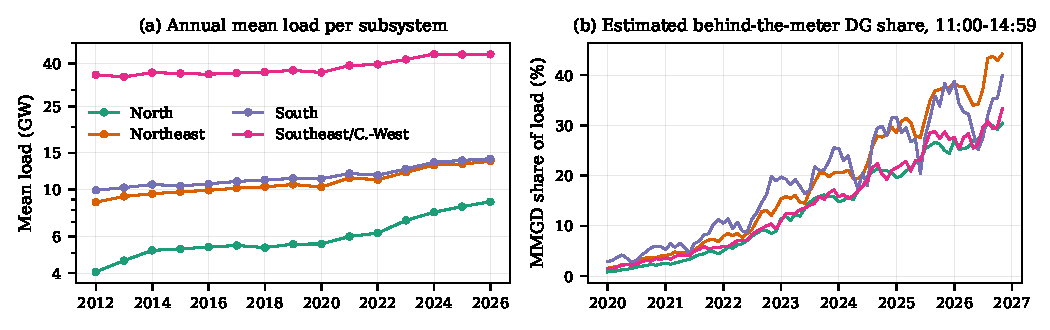
\includegraphics[width=\textwidth]{figures/fig_data.pdf}
\caption{(a) Annual mean hourly load of the four SIN subsystems (log scale; 2026 up to November 4). (b) Monthly mean share of the verified global load supplied by behind-the-meter distributed generation (MMGD) between 11:00 and 14:59, as estimated by ONS.}
\label{fig:data}
\end{figure*}

\begin{figure*}[!t]
\centering
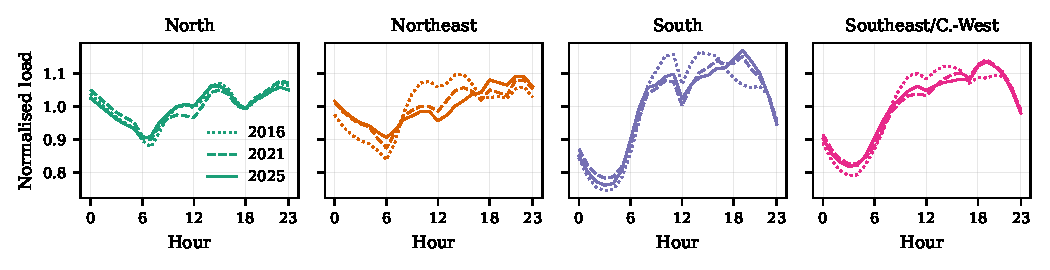
\includegraphics[width=\textwidth]{figures/fig_profiles.pdf}
\caption{Average weekday load profile, normalised by its daily mean, for 2016, 2021 and 2025.}
\label{fig:profiles}
\end{figure*}
